\documentclass[journal,hidelinks]{IEEEtran}
\usepackage[utf8]{inputenc}
\usepackage[
  pdftitle={Course Project -- Initial Phase},
  pdfauthor={Andrei Purcarus},
  pdfsubject={ECSE-534 -- Analog Microelectronics}
]{hyperref}
\usepackage{graphicx}
\usepackage[all]{hypcap}
\usepackage{cleveref}
\usepackage{indentfirst}
\usepackage[per-mode=symbol]{siunitx}
\usepackage{amsmath}

\title{ECSE-534 \\ Analog Microelectronics \\ Course Project -- Initial Phase}
\author{Andrei~Purcarus,~260631911,~\IEEEmembership{McGill~University} \\ \href{mailto:andrei.purcaruscraciun@mail.mcgill.ca}{andrei.purcaruscraciun@mail.mcgill.ca}}

\begin{document}
\sloppy

\maketitle

\begin{abstract}

A first order, single bit, $\Delta \Sigma$ A/D converter was designed, simulated, and analyzed using MATLAB and Cadence. This converter was required to achieve a peak SNDR of at least $\SI{60}{\deci\bel}$ with a bandwidth of $\SI{38.22}{\kilo\hertz}$ and a full scale input range of $\pm \SI{0.2}{\volt}$. To meet these goals, a sampling frequency of $\SI{10}{\mega\hertz}$ was used, which resulted in a peak SNDR of $\SI{76.69}{\deci\bel}$ in a system level simulation and of $\SI{55.7223}{\deci\bel}$ in a circuit level simulation. Given that the circuit level simulation SNDR does not meet the specifications, several avenues of inquiry to pursue in the final phase of the project were also suggested.

\end{abstract}

\section{Introduction}

\IEEEPARstart{T}{his} report follows the design, simulation, and analysis of a first order, single bit, low pass $\Delta \Sigma$ A/D converter using a 0.13 micron process from IBM. We used MATLAB and Simulink to perform system level simulations and Cadence and Analog Environment to perform circuit level simulations in said process. The converter was required to meet the following specifications:
\begin{itemize}
  \item Bandwidth: $(1 + \alpha) \cdot \SI{20}{\kilo\hertz}$, where $\alpha =$ (last 3 digits of student ID) / 1000.
  \item SNDR (peak): \SI{60}{\deci\bel} ($>$ 10 bits).
  \item Input Voltage Range: $\SI{\pm 0.2}{\volt}$ relative to AGND.
  \item Power Dissipation: Minimum.
\end{itemize}

In addition, we were assigned a supply voltage of $\SI{1.2}{\volt}$ and an analog ground voltage of AGND $= \SI{0.6}{\volt}$. To meet these specifications, we first performed a system level simulation using MATLAB and Simulink to determine the high level parameters required. Then, we mapped the system to a circuit and performed a circuit level simulation using Cadence and Analog Environment. Finally, we analyzed the performance of the converter and verified if it meets the specifications.

\section{System Level Simulation}

We first simulated the ADC at the system level. We began by calculating the requirements of our system. From our student ID, we can determine that $\alpha = 0.911$, which means our bandwidth is $f_{3dB} = \SI{38.22}{\kilo\hertz}$. To compute our minimal SNR, we assume that the power of the noise in our system will be about equal to the power of the signal harmonics. Thus, we require SNR $= 2$ SNDR, or SNR $= \SI{63}{\deci\bel}$ at the minimum. We can therefore compute our desired oversampling rate as
\[ OSR = 10^{(SNR_{peak} - 2.61)/30} = 103.04 \]
Using this result, we can determine that our minimum sampling frequency must be
\[ f_s = 2 \  OSR \  f_{3dB} = \SI{7.88}{\mega\hertz} \]
To allow for some margin, we chose $f_s = \SI{10}{\mega\hertz}$.

Next, we set up the simulation in Simulink, as shown in \Cref{fig:sim_diagram}. We used a $\SI{0.2}{\volt}$ amplitude sine wave with a DC offset of $\SI{0.6}{\volt}$ as our input to the system, and we sampled this input at a rate of $\SI{10}{\mega\hertz}$. We also used $\SI{1}{\kilo\hertz}$ bins for all SNDR calculations.

\begin{figure}[!htb]
  \centering
  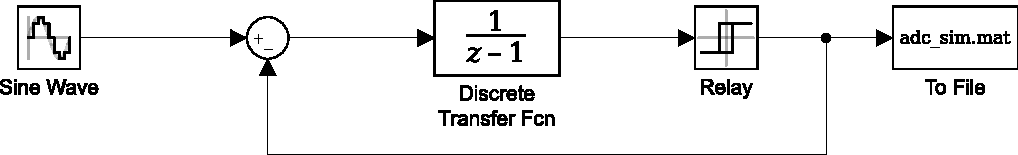
\includegraphics[width=\columnwidth]{simulation/adc_sim.pdf}
  \caption{A system level block diagram of the $\Delta \Sigma$ A/D converter.}
  \label{fig:sim_diagram}
\end{figure}

To find our peak SNDR, we first set the relay outputs to $\SI{0.4}{\volt}/\SI{0.8}{\volt}$ and swept the input frequency. The results are shown in \Cref{fig:sim_freq}. From this plot, we can see that the frequency with the best SNDR is around $\SI{20}{\kilo\hertz}$. This can be explained by the fact that the first harmonic for this input frequency occurs at $\SI{40}{\kilo\hertz}$, which is outside our bandwidth and hence does not add distortion.

\begin{figure}[!htb]
  \centering
  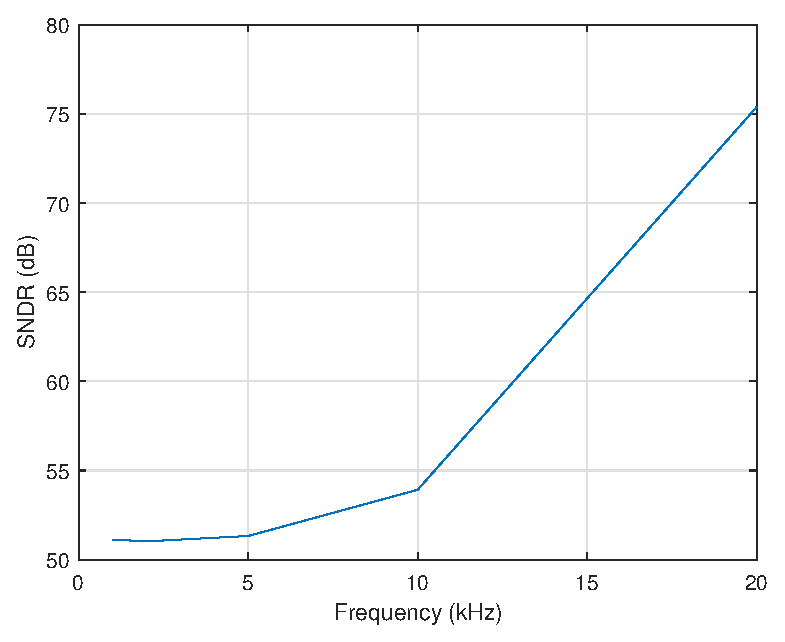
\includegraphics[width=0.8\columnwidth]{simulation/adc_sim_freq.eps}
  \caption{SNDR vs. input frequency for the $\Delta \Sigma$ A/D converter with the relay outputs set at $\SI{0.4}{\volt}/\SI{0.8}{\volt}$.}
  \label{fig:sim_freq}
\end{figure}

Next, we kept the input frequency at $\SI{20}{\kilo\hertz}$ and swept the amplitude of the relay output around a DC offset of $\SI{0.6}{\volt}$. The results are shown in \Cref{fig:sim_vo}. From this plot, we can see that the peak SNDR of $\SI{76.69}{\deci\bel}$ occurs when the relay output amplitude is $\SI{0.4}{\volt}$, corresponding to relay outputs of $\SI{0.2}{\volt}/\SI{1.0}{\volt}$.

\begin{figure}[!htb]
  \centering
  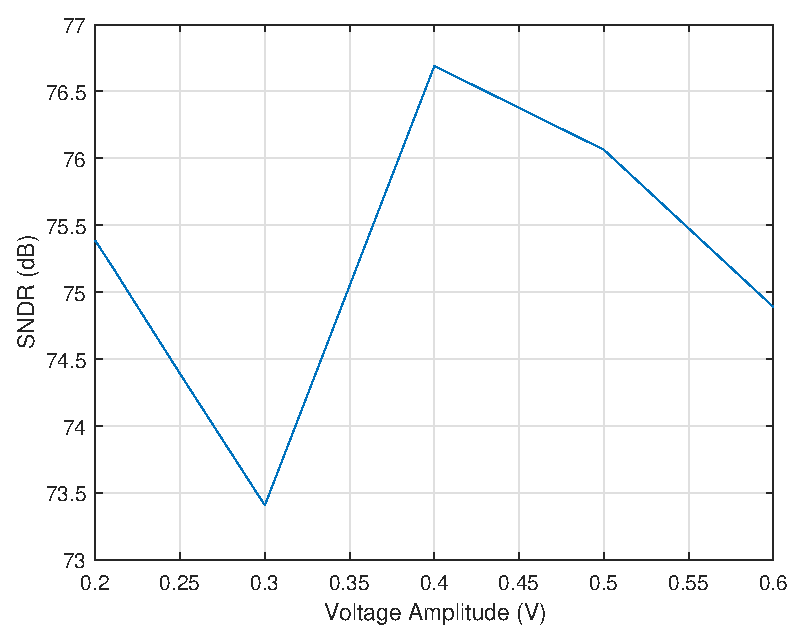
\includegraphics[width=0.8\columnwidth]{simulation/adc_sim_vo.eps}
  \caption{SNDR vs. relay output amplitude for the $\Delta \Sigma$ A/D converter with the input frequency set at $\SI{20}{\kilo\hertz}$.}
  \label{fig:sim_vo}
\end{figure}

Thus, we chose to use an input frequency of $\SI{20}{\kilo\hertz}$ and a relay output amplitude of $\SI{0.4}{\volt}$ for our design. The power spectral density of the output with these settings is shown in \Cref{fig:sim_psd}. This plot clearly shows that the output has a peak at the input frequency of $\SI{20}{\kilo\hertz}$, with the first harmonic occurring outside of our bandwidth at $\SI{40}{\kilo\hertz}$.

\begin{figure}[!htb]
  \centering
  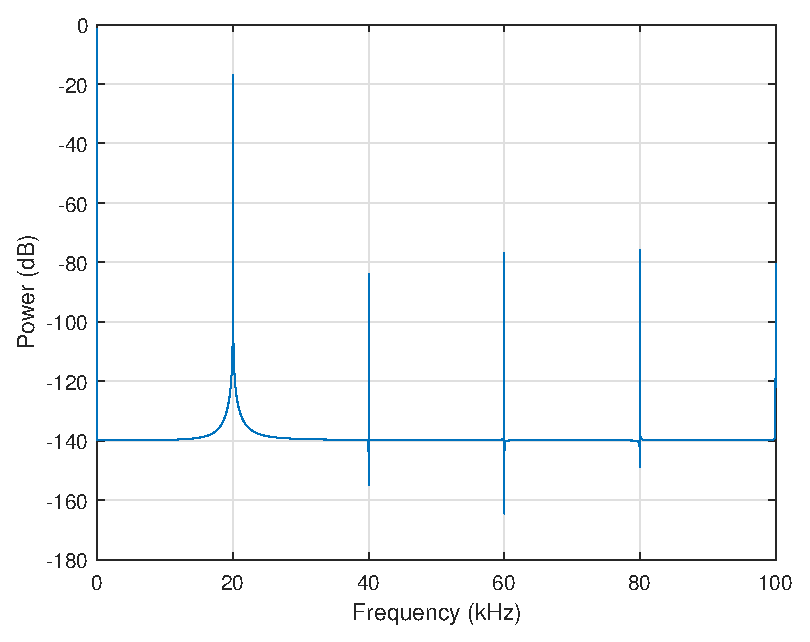
\includegraphics[width=0.8\columnwidth]{simulation/adc_sim_psd.eps}
  \caption{Power spectral density for the output of the $\Delta \Sigma$ A/D converter with the input frequency set at $\SI{20}{\kilo\hertz}$ and the relay outputs set at $\SI{0.2}{\volt}/\SI{1.0}{\volt}$.}
  \label{fig:sim_psd}
\end{figure}

\section{Circuit Level Simulation}

We next mapped the system to a circuit using Cadence. We reused the operational amplifier designed in Assignments \#2 and \#3 to implement an integrator. We also used a modified version of the operational amplifier with the compensation network removed to implement a comparator. These are shown in \Cref{fig:adc} as $U_1$ and $U_2$ respectively. The remaining components required digital logic. As a starting point, we used $\SI{10}{\micro\meter}/\SI{0.12}{\micro\meter}$ NMOS transistors and $\SI{25}{\micro\meter}/\SI{0.12}{\micro\meter}$ PMOS transistors for all our digital logic.

We first implemented a NOT gate and a NOR gate to provide building blocks for our other circuit elements. Schematics of these implementations are shown in \Cref{fig:not_gate,fig:nor_gate}. Then, we used the NOT gate to implement a basic transmission gate, as shown in \Cref{fig:transmission_gate}.

\begin{figure}[!htb]
  \centering
  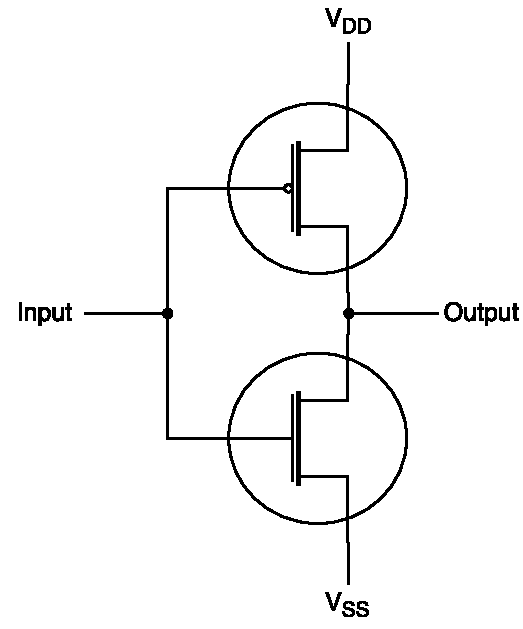
\includegraphics[height=0.5\columnwidth]{diagrams/not_gate.pdf}
  \caption{A schematic of a NOT gate (inverter) implementation.}
  \label{fig:not_gate}
\end{figure}

\begin{figure}[!htb]
  \centering
  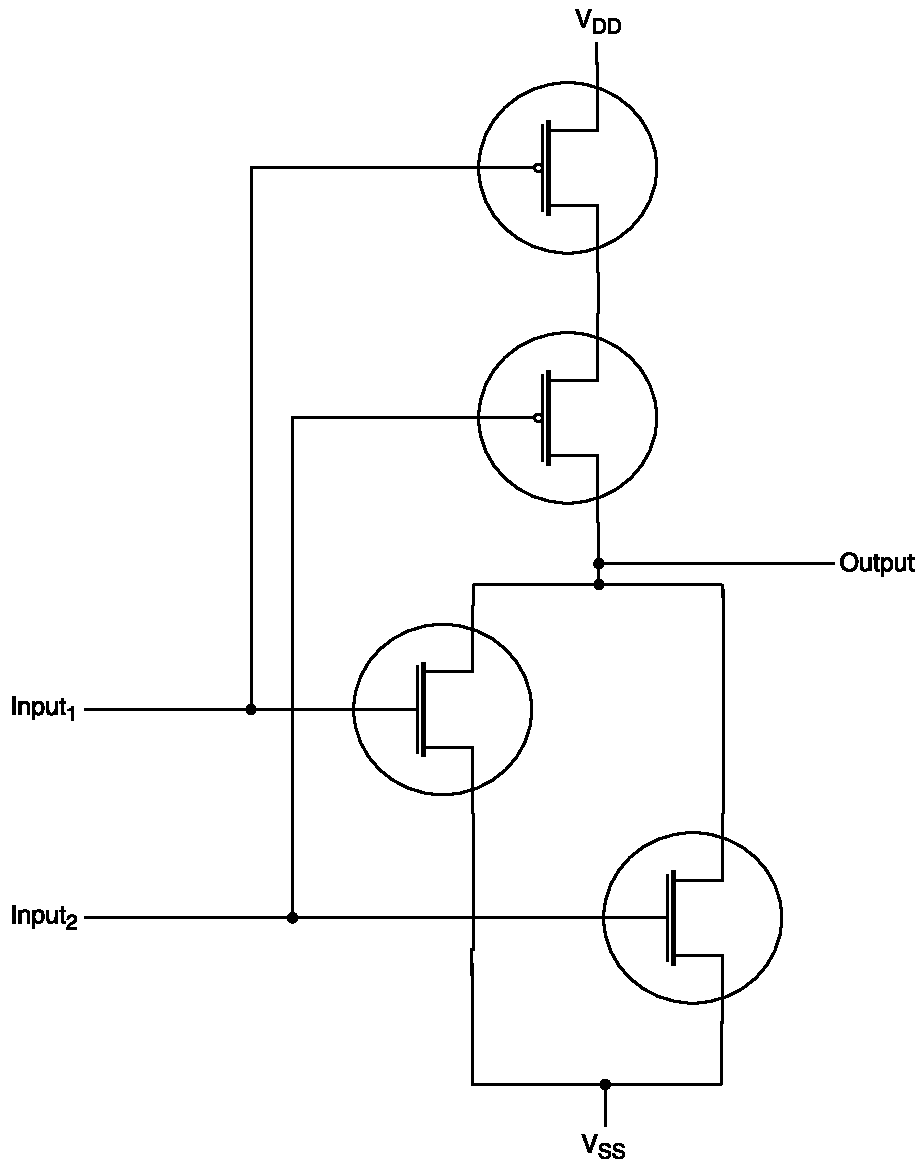
\includegraphics[height=0.8\columnwidth]{diagrams/nor_gate.pdf}
  \caption{A schematic of a two-input NOR gate implementation.}
  \label{fig:nor_gate}
\end{figure}

\begin{figure}[!htb]
  \centering
  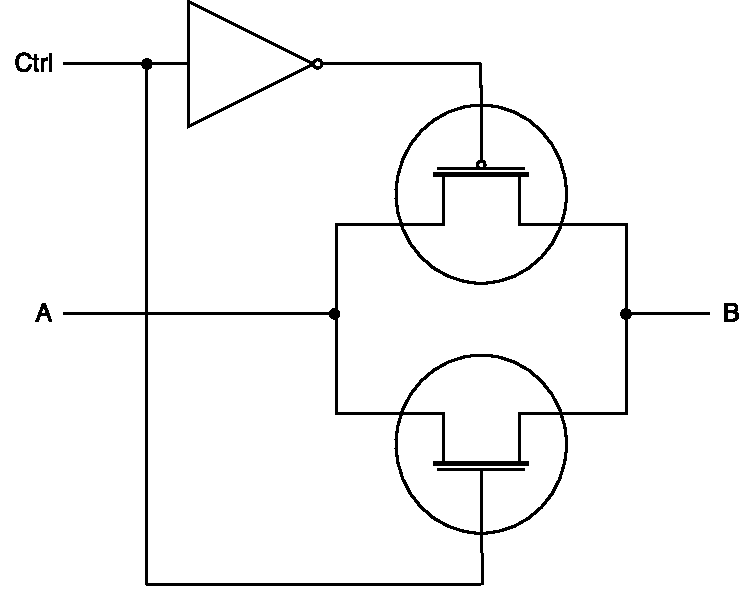
\includegraphics[height=0.5\columnwidth]{diagrams/transmission_gate.pdf}
  \caption{A schematic of a transmission gate implementation.}
  \label{fig:transmission_gate}
\end{figure}

\begin{figure*}[!htb]
  \centering
  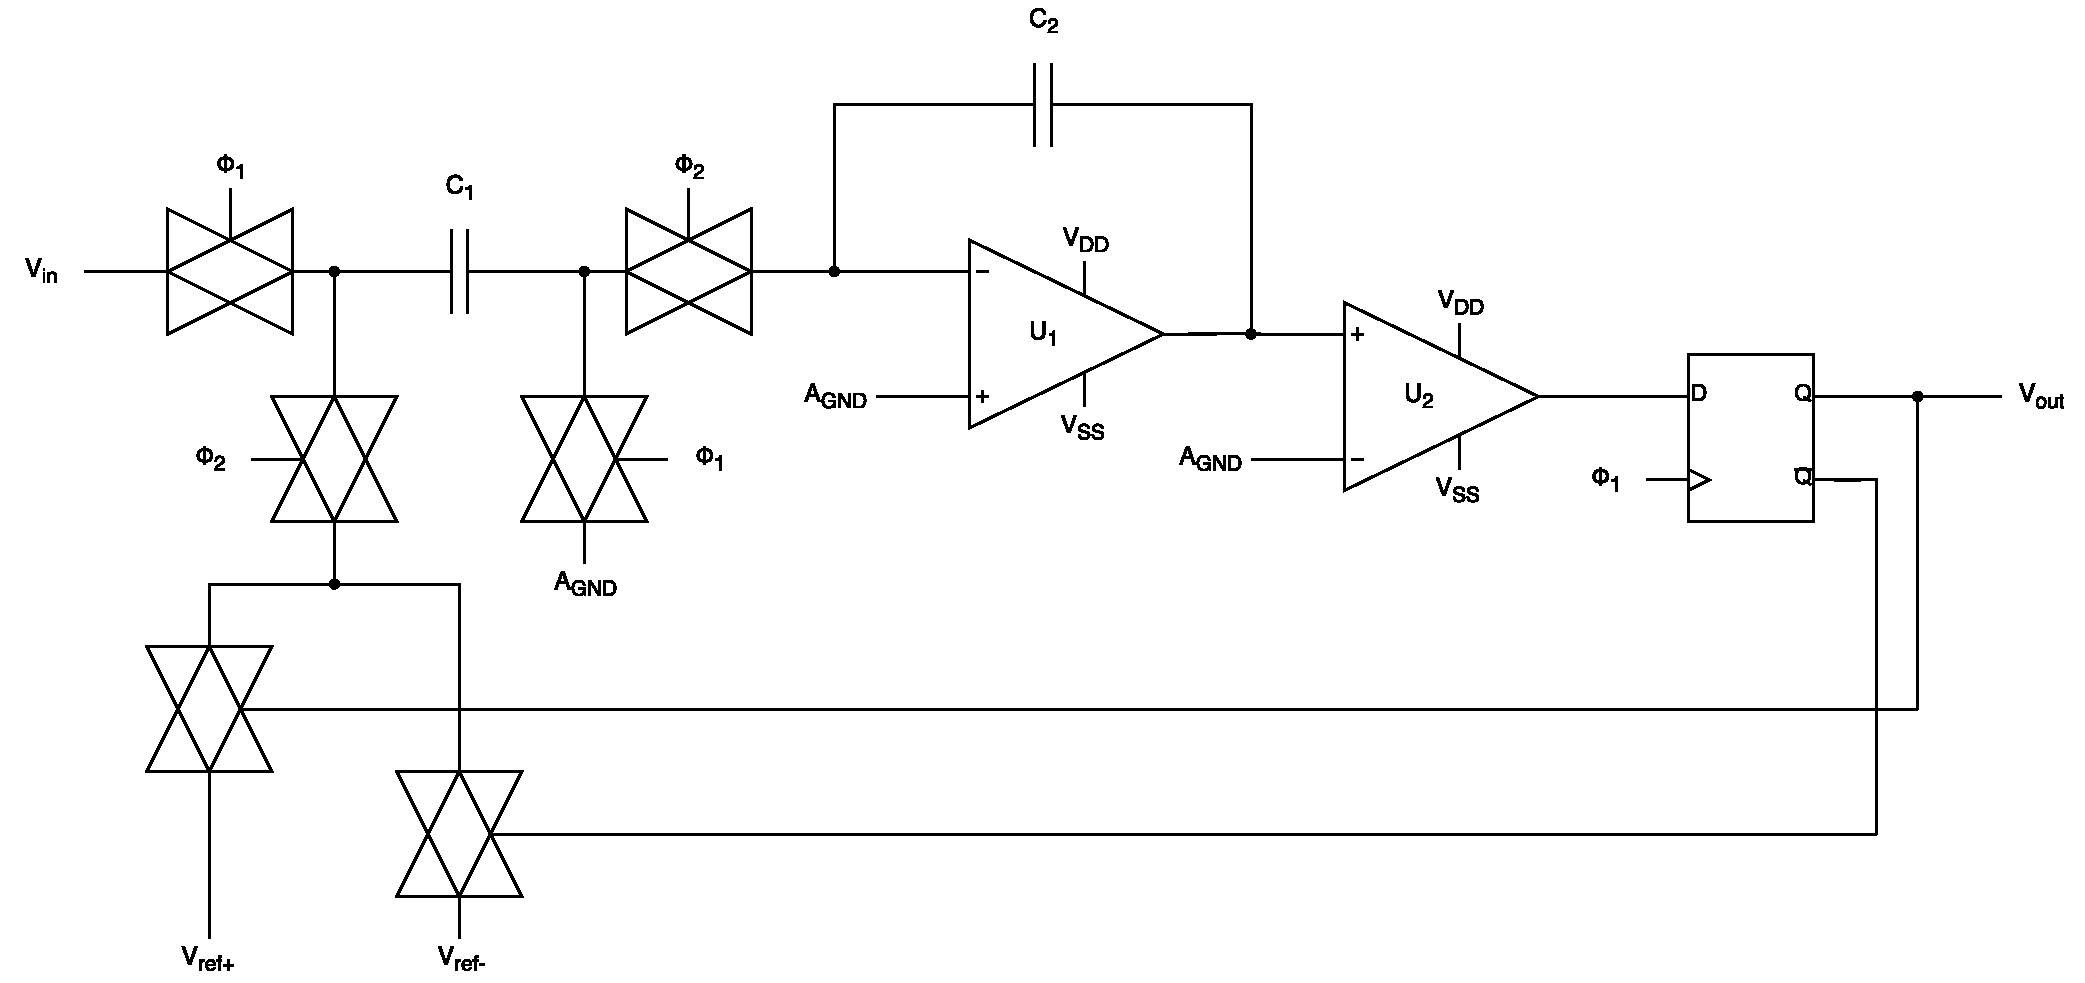
\includegraphics[width=\textwidth]{diagrams/adc.pdf}
  \caption{A schematic of the $\Delta \Sigma$ A/D converter.}
  \label{fig:adc}
\end{figure*}

Then, we implemented a D flip-flop in order to add a sampling element to our circuit. A schematic of this implementation is shown in \Cref{fig:ff}. This flip-flop is triggered by the falling edge of the clock signal.

\begin{figure}[!htb]
  \centering
  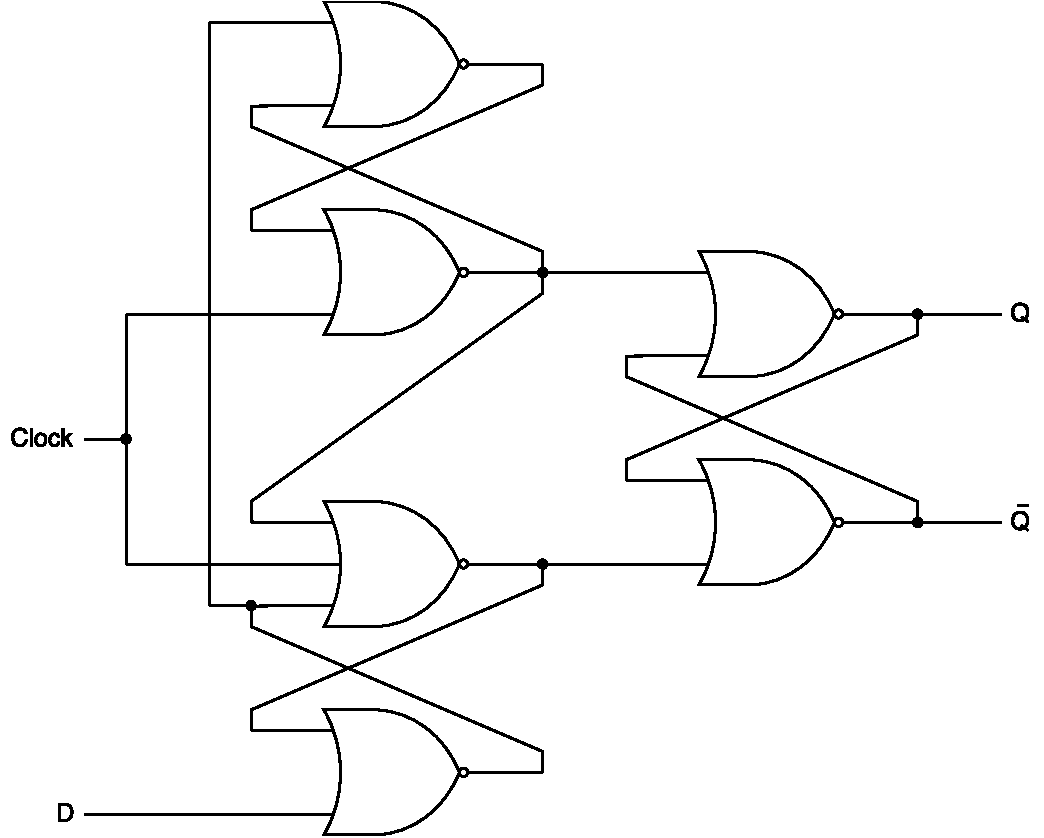
\includegraphics[width=0.8\columnwidth]{diagrams/ff.pdf}
  \caption{A schematic of a D flip-flop implementation.}
  \label{fig:ff}
\end{figure}

Finally, we implemented the circuit shown in \Cref{fig:clock} to generate a 2-phase clock signal that we could use to operate our switched capacitor circuit. We achieved this by simply negating the clock to provide the second phase, and then using an SR latch and a series of buffers to ensure that the two phases never overlap.

\begin{figure}[!htb]
  \centering
  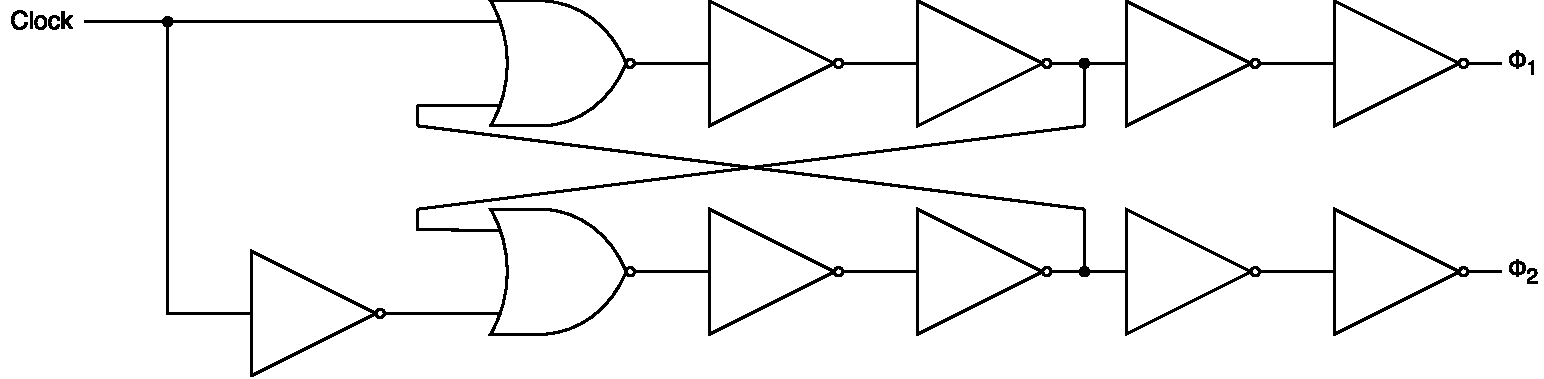
\includegraphics[width=\columnwidth]{diagrams/clock.pdf}
  \caption{A schematic of a 2-phase clock generator implementation.}
  \label{fig:clock}
\end{figure}

With these subcomponents in hand, we then implemented the complete ADC, as shown in \Cref{fig:adc}. We chose values of $C_1 = C_2 = \SI{0.5}{\pico\farad}$ as a starting point, making sure to match them in order to implement a discrete integrator. In addition, we used the reference voltages of $V_{ref+} = \SI{1.0}{\volt}$ and $V_{ref-} = \SI{0.2}{\volt}$ that were previously found to give the best SNDR.

We next performed a transient analysis of the circuit. As we did in our system level simulation, we used a $\SI{10}{\mega\hertz}$ clock and a $\SI{0.2}{\volt}$ amplitude, $\SI{20}{\kilo\hertz}$ sine wave input signal. We then ran the simulation for $\SI{2}{\milli\second}$, which allowed us to get $\SI{500}{\hertz}$ bins in our FFT. One issue we encountered was that the FFT expects uniform sampling while Analog Environment produces non-uniformly sampled outputs. To fix this, we set the \verb|strobeperiod| option of the transient simulation to $\SI{10}{\nano\second}$, which produces a uniformly sampled output and gives us 10 points per period of the sampling clock.

A portion of the results are shown in \Cref{fig:debug}. In this plot, we can see the integrator output for a given input signal. We see that in this case, with the signal being greater than analog ground, the negative error when the DAC outputs $\SI{1.0}{\volt}$ produces small steps downward, which eventually leads to crossing the analog ground line. At that point, the DAC output switches to $\SI{0.2}{\volt}$, and the larger positive error causes the integrator output to rise rapidly above the analog ground line. This illustrates how the ADC produces an output whose mean value is correlated with the value of the input signal.

\begin{figure}[!htb]
  \centering
  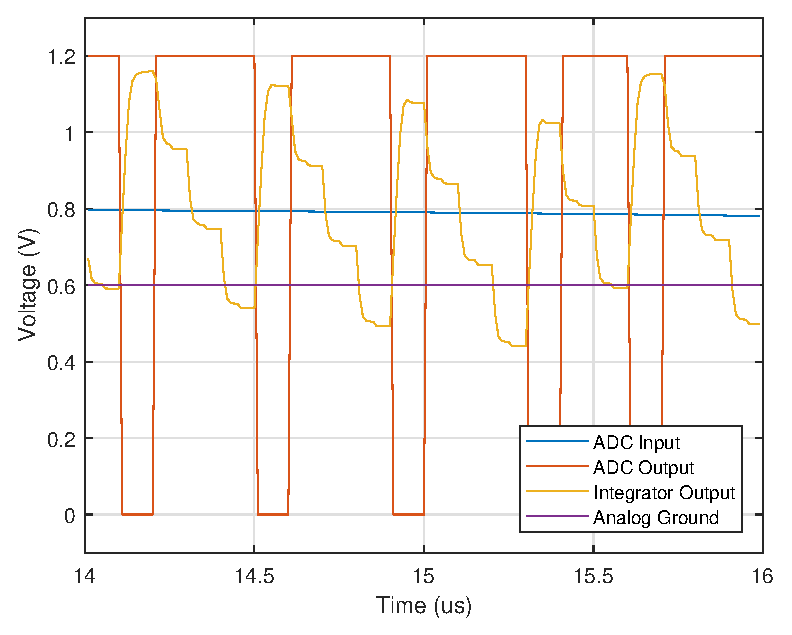
\includegraphics[width=0.8\columnwidth]{circuit/adc_cir_debug.eps}
  \caption{Transient response of the $\Delta \Sigma$ A/D converter with the input frequency set at $\SI{20}{\kilo\hertz}$ and the relay outputs set at $\SI{0.2}{\volt}/\SI{1.0}{\volt}$.}
  \label{fig:debug}
\end{figure}

We next processed the simulation data over the entire $\SI{2}{\milli\second}$ and obtained a SNDR of $\SI{55.7223}{\deci\bel}$ over our bandwidth of $\SI{38.22}{\kilo\hertz}$. We used $\SI{1}{\kilo\hertz}$ bins to match the system level simulation. A plot of the power spectral density we obtained is shown in \Cref{fig:cir_psd}.

\begin{figure}[!htb]
  \centering
  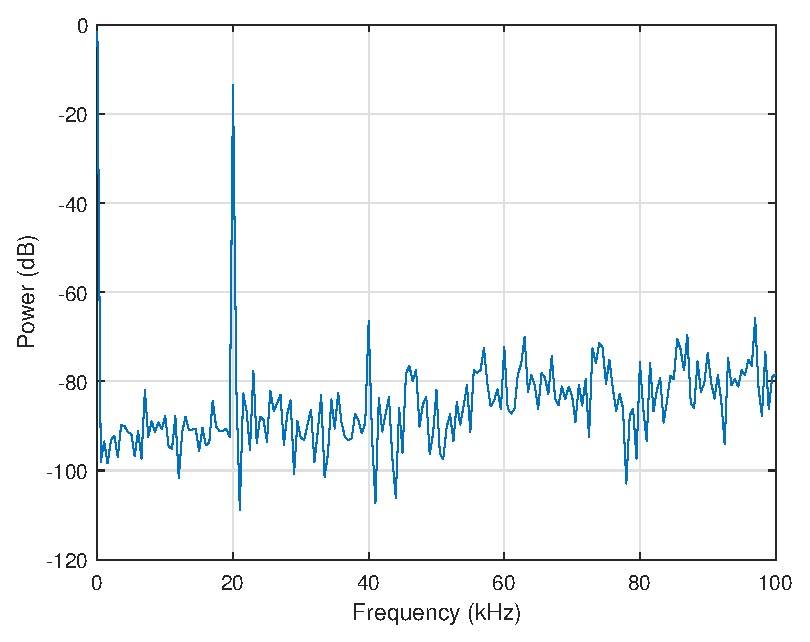
\includegraphics[width=0.8\columnwidth]{circuit/adc_cir_psd.eps}
  \caption{Power spectral density for the output of the $\Delta \Sigma$ A/D converter with the input frequency set at $\SI{20}{\kilo\hertz}$ and the relay outputs set at $\SI{0.2}{\volt}/\SI{1.0}{\volt}$.}
  \label{fig:cir_psd}
\end{figure}

Finally, we measured the power supply current and multiplied it by $V_{DD} = \SI{1.2}{\volt}$ in order to calculate the circuit's power dissipation. The results are shown in \Cref{fig:cir_power}. We can see that large spikes occur when the circuit's digital components are switching. Integrating the curve and dividing by the interval yields an average power dissipation of $\SI{195}{\micro\watt}$.

\begin{figure}[!htb]
  \centering
  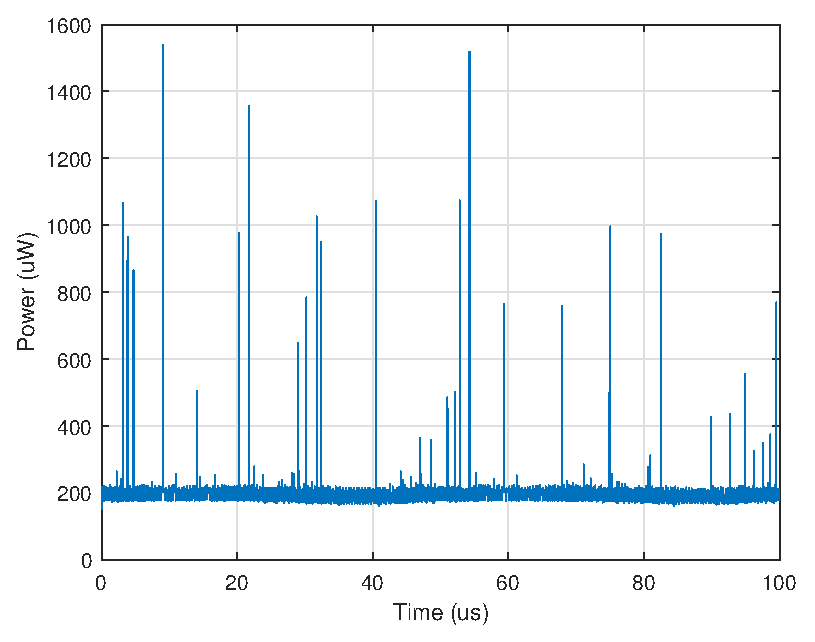
\includegraphics[width=0.8\columnwidth]{circuit/adc_cir_power.eps}
  \caption{Power dissipation of the $\Delta \Sigma$ A/D converter with the input frequency set at $\SI{20}{\kilo\hertz}$ and the relay outputs set at $\SI{0.2}{\volt}/\SI{1.0}{\volt}$.}
  \label{fig:cir_power}
\end{figure}

\section{Analysis}

In terms of SNDR, the circuit level simulation produced a much lower result than the system level simulation. In fact, the value of $\SI{55.7223}{\deci\bel}$ obtained is below the spec of $\SI{60}{\deci\bel}$, and far below the system level simulation value of $\SI{76.69}{\deci\bel}$. This can be explained by several factors. As shown in \Cref{fig:sim_psd,fig:cir_psd}, the noise floor for the system level simulation is around $\SI{-140}{\deci\bel}$, while it is around $\SI{-90}{\deci\bel}$ for the circuit level simulation. This could be a result of additional quantization error, or a result of additional noise being introduced by the other components in the circuit. Since the system level simulation meets the specification, it seems more likely that the latter is the cause. However, more investigation is required for the final phase.

Several possible improvements that we will examine include the use of a 4-phase clock system and the use of bootstrapped transmission gates to reduce charge injection and improve linearity. In addition, we will look at second order effects to try to determine the principal causes of the reduced SNDR.

In terms of power dissipation, we were not given an explicit requirement. However, we can evaluate our implementation by comparing our average power dissipation of $\SI{195}{\micro\watt}$ to the Assignment 2 maximum of $\SI{200}{\micro\watt}$. This comparison shows that our power dissipation is quite low, given that our combined circuit consumes less power on average than the maximum we were given for a single operational amplifier. However, there are some improvements that can be made. In particular, the bias circuits of the operational amplifier and the comparator should be merged in order to save on power and silicon area. This will also improve the layout by reducing the need to lay out multiple current references.

\section{Conclusions}

In conclusion, we designed, simulated, and analyzed a first order, single bit, $\Delta \Sigma$ A/D converter using MATLAB and Cadence. To meet our specifications of a $\SI{38.22}{\kilo\hertz}$ bandwidth and a peak SNDR of at least $\SI{60}{\deci\bel}$, we used a sampling frequency of $\SI{10}{\mega\hertz}$. We then found that our peak SNDR occurs when the input frequency is $\SI{20}{\kilo\hertz}$ and our DAC output voltage levels are $\SI{0.2}{\volt}/\SI{1.0}{\volt}$. With these parameters, our system level simulation yielded a SNDR of $\SI{76.69}{\deci\bel}$, while our circuit level simulation yielded a SNDR of $\SI{55.7223}{\deci\bel}$. Given that our circuit level simulation SNDR does not meet the specifications, we also suggested several avenues of inquiry to pursue for the final phase of the project.

\bibliographystyle{IEEEtran}
\bibliography{IEEEabrv,references}

\end{document}
